% Main latex file for the boxcom howto.

% The left footer on the normal pagestyle pages
\newcommand{\normalleftfoot}{This is my stuff}

% The right footer on the normal pagestyle pages
\newcommand{\normalrightfoot}{More stuff}


% The manual_template controls page layout and things like the logo
% in each page footer.
\input{doctools/latex/manual_template.tex}  
\input{doctools/latex/mycommands.tex} % Some useful commands
\input{doctools/latex/units.tex} % Macros for pretty measurement units

% Some text is inserted in drafts that shouldn't be in the released
% version.  For example, some figures have their filenames printed in
% the draft version.  See the \draftnote command in mycommands to
% insert text like this.
\newcommand{\isdraft}{1} % Choose 1 for draft, 0 for release

% isforme
% Choose 1 for in-house use, 0 for outside.  The in-house manual
% will contain the dollar-sign calibration commands
\newcommand{\isforme}{1} % Choose 1 for internal, 0 for outside

% Figure search path
\graphicspath{
              {figs/} % Figures drawn with xfig
              }

% These commands cause  usr_commands.idx and srs_commands.idx to be
% generated when latex is run on this file and the multind.sty file
% is pulled in (by manual_template)
\makeindex{user_cmds_index}
\makeindex{internal_cmds_index}

\begin{document}


%\doublespacing %set double spacing

% Title page
\thispagestyle{empty}   % First page does not need headers and footers
\vspace*{\fill}
\begin{center}
{\huge boxcom howto}\\
\today
\end{center}
\vspace*{\fill}
\clearpage


% Table of contents page
\pagestyle{toc} % Set the toc page style
\tableofcontents{}
\clearpage{}    % There must be a \clearpage to end a page style

\pagestyle{normal} % Set the normal page style

%%%%%%%%%%%%%%%%%%%%%%%%%%%%%%%%%%%%%%%%%%%%%%%%%%%%%%%%%%%%%%%%%%%%%
% The USB board
%
% Subsections:
% 
%%%%%%%%%%%%%%%%%%%%%%%%%%%%%%%%%%%%%%%%%%%%%%%%%%%%%%%%%%%%%%%%%%%%%
\section{USB board}

\subsection{Making connections}
Figure \ref{fig:panel_switch_wiring} shows how the front panel power
switch should be wired.

\begin{figure}[ht]
  \begin{center}
    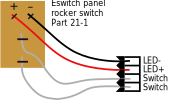
\includegraphics[clip,scale=1]{figs/panel_switch_wiring}
    \caption{Panel switch wiring \label{fig:panel_switch_wiring}}
  \end{center}
\end{figure}

Figure \ref{fig:post_cable} shows how to make the cable connecting the
monitored 3.3V output to the front panel binding posts.
\begin{figure}[ht]
  \begin{center}
    
\includegraphics[clip,scale=1]{figs/post_cable}
    \caption{Panel switch wiring \label{fig:post_cable}}
  \end{center}
\end{figure}


\clearpage{}
\subsection{Board checkout}


\subsubsection{Voltage rails}
Use table \ref{tab:usb_rails} to keep track of voltage rails.

\begin{table}[ht]
  \begin{center}
    \begin{tabular}{|c|c|c|c|}
      \hline
      Net name &Test points &Acceptable &Actual\\
      \hline \hline
      $\mathrm{V_{bus}}$ &TP100 vs.\ TP101 &\cwksentry{1in}{4.5V $\rightarrow$ 5.5V} 
        &\cwksentry{1in}{} \\
      \hline
      $\mathrm{+3.3V_{aux}}$ &TP400 vs.\ TP401 &\cwksentry{1in}{3.14V $\rightarrow$ 3.45V} 
        &\cwksentry{1in}{} \\
      \hline
      $\mathrm{+3.3V_{mon}}$ &TP500 vs.\ TP401 &\cwksentry{1in}{3.14V $\rightarrow$ 3.45V} 
        &\cwksentry{1in}{} \\
      \hline
    \end{tabular}
    \caption{Voltage rail checkout table for the USB
      board.\label{tab:usb_rails}}
  \end{center}
\end{table}

\subsubsection{Current monitor}
The current monitor output at J500 will have a fixed DC output, since
the voltage regulator following it always draws at least 1mA. As
illustrated in figure \ref{fig:monitor_test}, the slope set in
hardware should give $\Delta \mathrm{V_{out}}$ = 1V for each
additional 10mA of current draw from J501.  Since the voltage output
from J501 is controlled at 3.3V, a test load of 3.3k$\Omega$ should
increase the voltage at J500 by 100mV.

\begin{figure}[ht]
  \begin{center}
    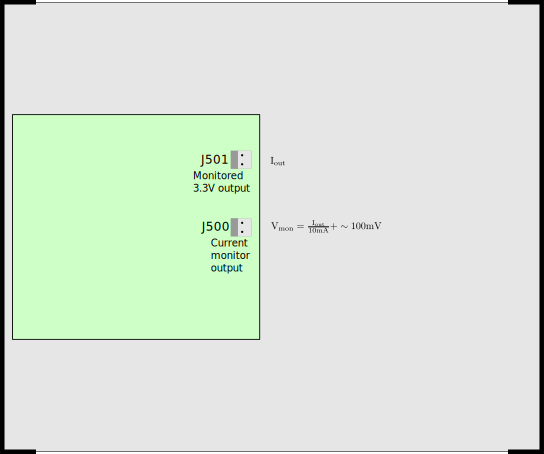
\includegraphics[clip,scale=.5]{figs/monitor_test}
    \caption{The output connectors used during the current monitor test.\label{fig:monitor_test}}
  \end{center}
\end{figure}

\begin{table}[ht]
  \begin{center}
    \begin{tabular}{|c|c|c|}
      \hline
      Load applied to J501 & Acceptable $\mathrm{V_{out}}$ at J500 & Measured $\mathrm{V_{out}}$ at J500\\
      \hline\hline
      Open                 &90mV $\rightarrow$ 110mV &\wksentry{2cm}{$\mathrm{V_{out,o}} =$}\\
      \hline
      3.3k$\Omega$         &\cwksentry{3cm}{$\mathrm{V_{out,o}}$ + 100mV} &\\
      \hline
    \end{tabular}
    \caption{Passing voltage measurements for the current monitor test.\label{tab:monitor_test}}
  \end{center}
\end{table}

\subsubsection{Serial loopback}
The serial loopback test is a basic test of the USB/serial interface
and the RS-232 transceiver.  Make the breakout cable shown in figure
\ref{fig:db9_breakout}, then make connections to the board as shown in
figure \ref{fig:serial_loopback}.

\begin{figure}[ht]
  \begin{center}
    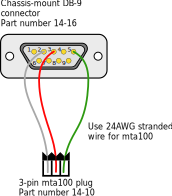
\includegraphics[clip,scale=1]{figs/usb_board_uart_to_db9}
    \caption{Wiring the DB9 breakout cable for the serial loopback
      test.\label{fig:db9_breakout}}
  \end{center}
\end{figure}

\begin{figure}[ht]
  \begin{center}
    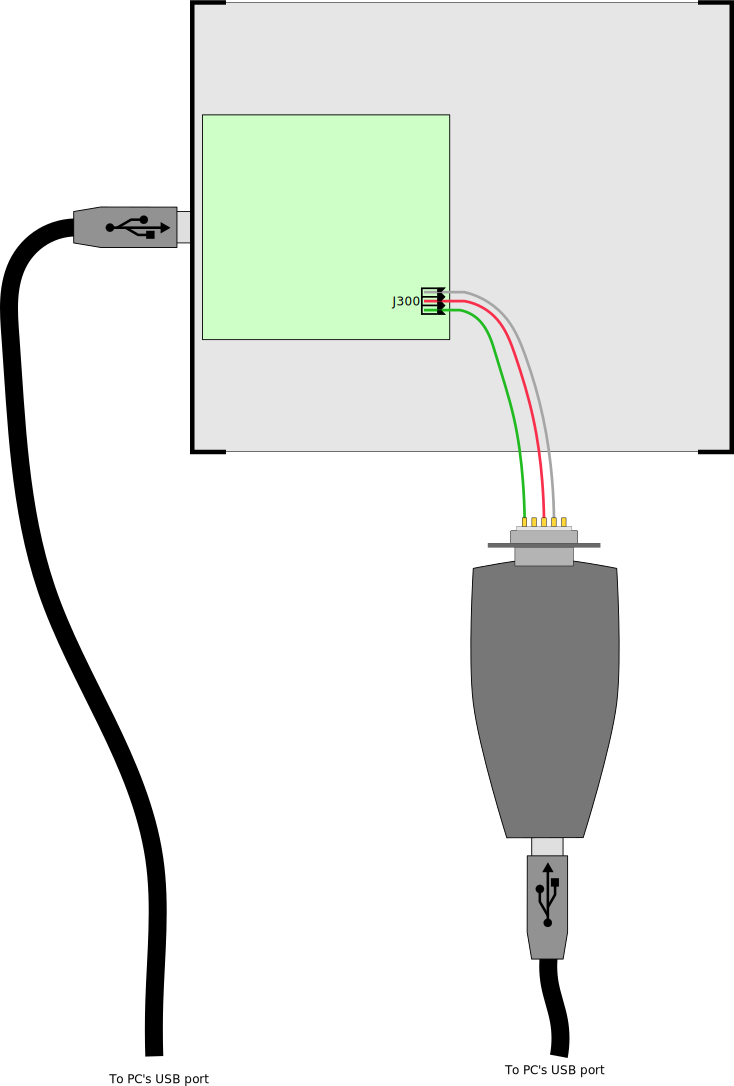
\includegraphics[clip,scale=0.5]{figs/serial_loopback_test}
    \caption{The setup for the serial loopback
      test.\label{fig:serial_loopback}}
  \end{center}
\end{figure}

The serial loopback test script is:
\begin{center}
  \texttt{boxcom/implement/data/scripts/tty\_loopback.py}
\end{center}
...and the test should pass at the speed listed in table
\ref{tab:loopback_test}.

\begin{table}[ht]
  \begin{center}
    \begin{tabular}{|c|c|}\hline
      Minimum passing baud  &Measured passing baud\\
      \hline\hline
      \cwksentry{5cm}{115200} &\cwksentry{5cm}{}\\
      \hline
    \end{tabular}
    \caption{Passing baud measurement for the serial loopback test.
      The usb board should be able to reliably pass the loopback test
      for data flowing in both directions at the minimum
      baud.\label{tab:loopback_test}}
  \end{center}
\end{table}

\clearpage{}
\subsection{Schematics}

% Control top-bottom placement with the vspace parameter
\begin{figure}[ht]
    \begin{center}
          \vspace{0.4cm}
          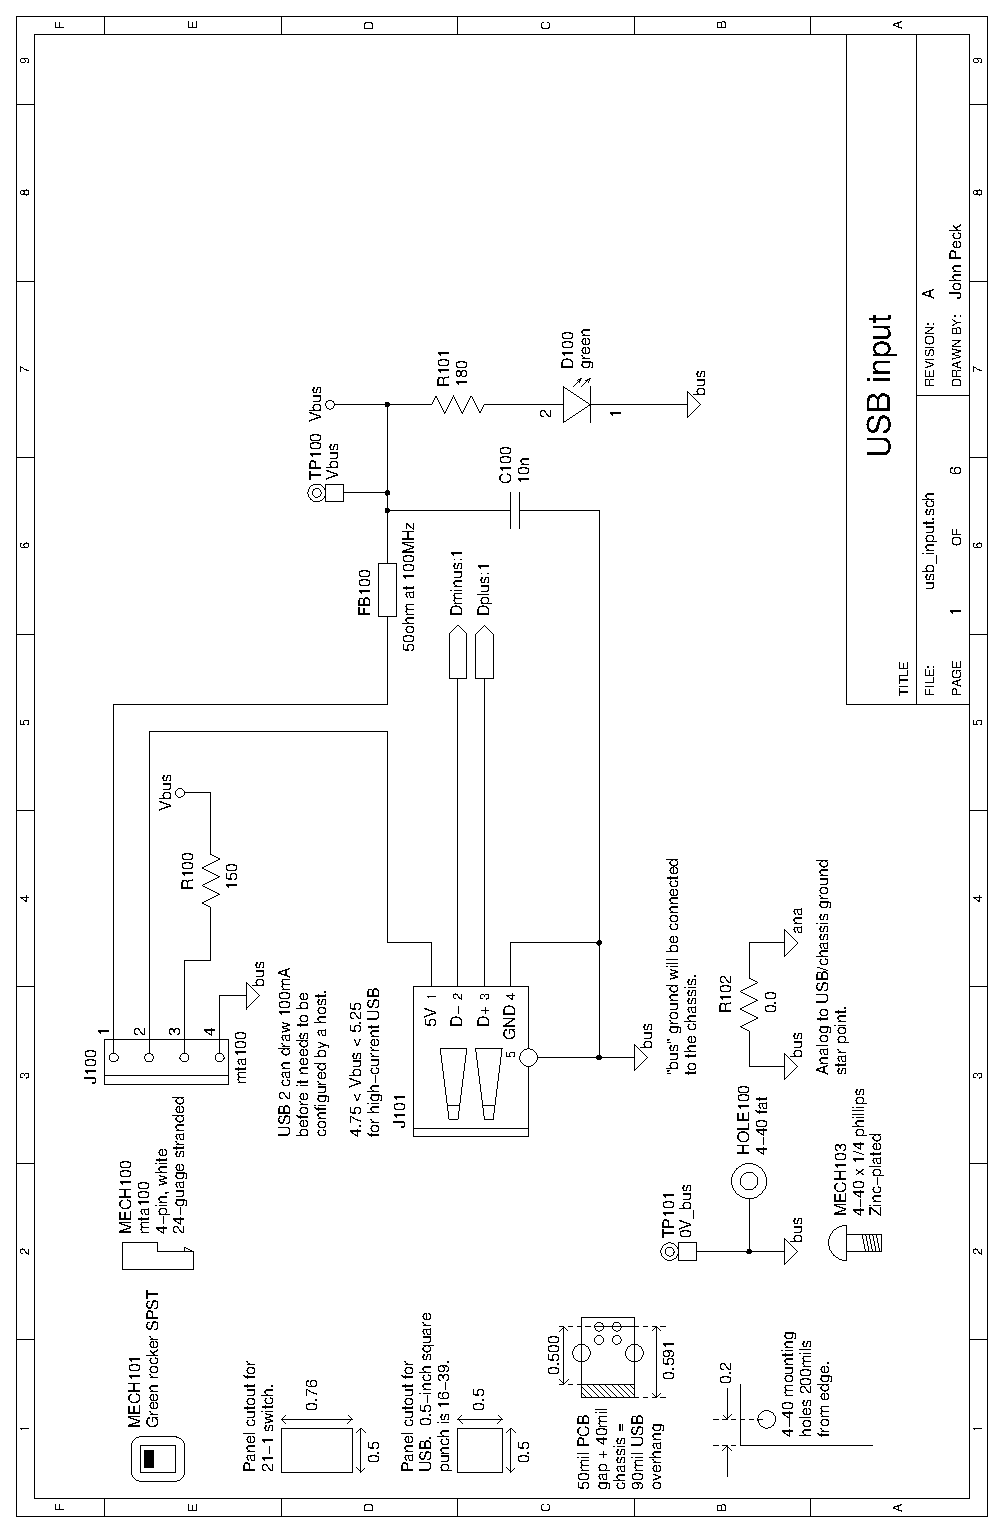
\includegraphics[clip,height=\textheight]
          {schematics/usb/usb_input}
          \label{sch:usb_input}
    \end{center} 
\end{figure}

\begin{figure}[ht]
    \begin{center}
          \vspace{0.4cm}
          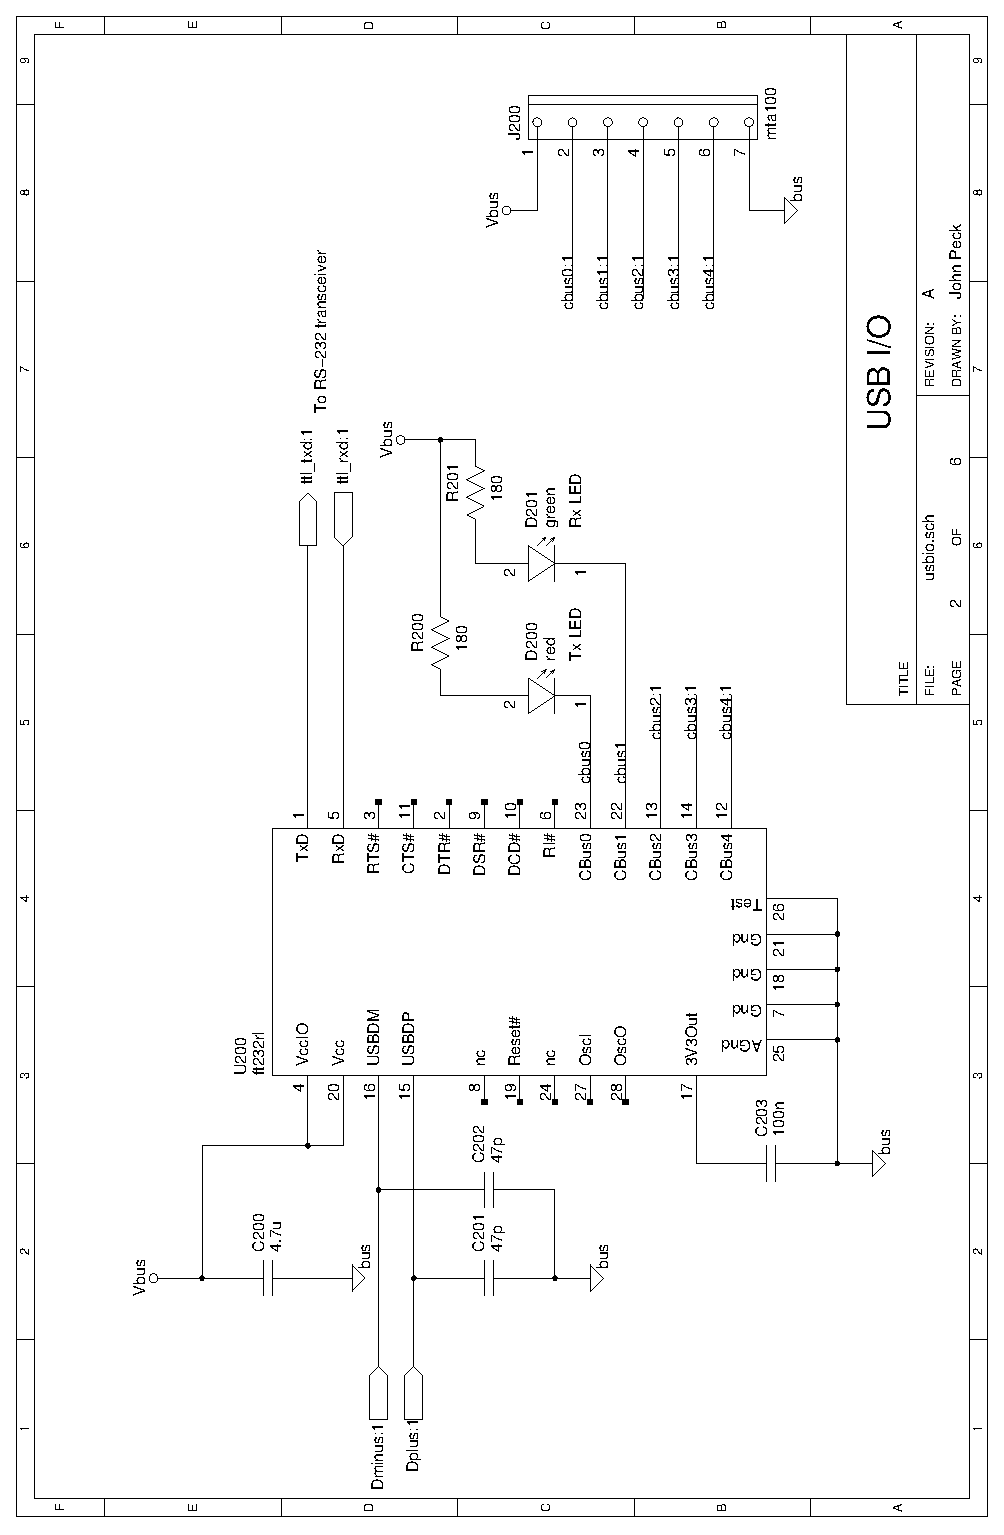
\includegraphics[clip,height=\textheight]
          {schematics/usb/usbio}
          \label{sch:usbio}
    \end{center} 
\end{figure}

\begin{figure}[ht]
    \begin{center}
          \vspace{0.4cm}
          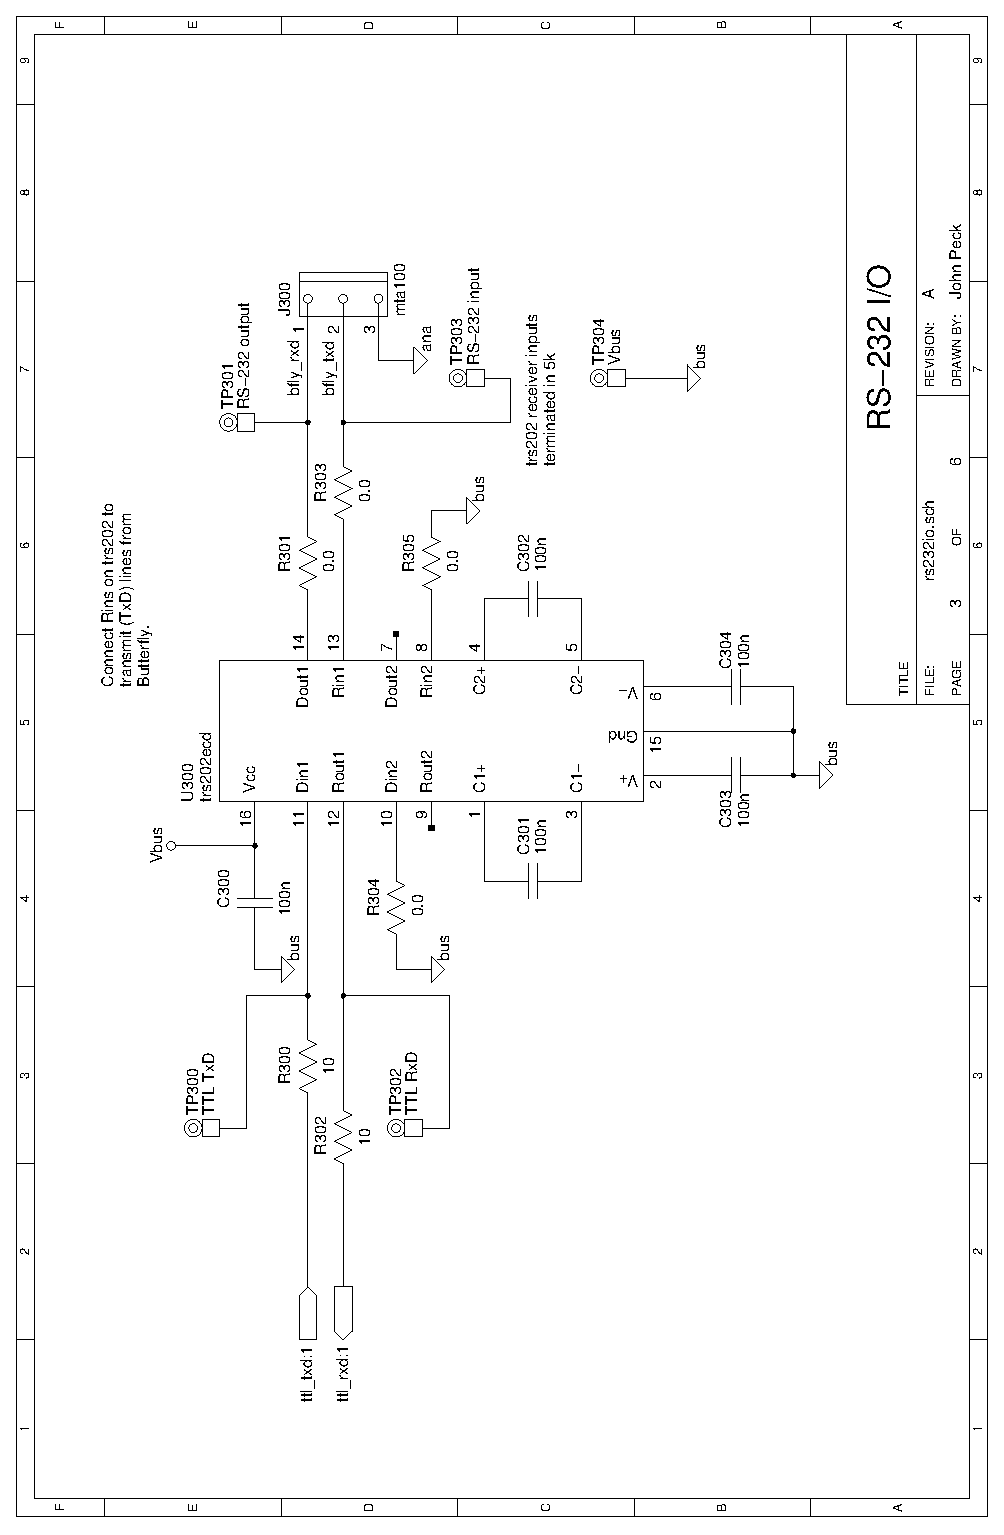
\includegraphics[clip,height=\textheight]
          {schematics/usb/rs232io}
          \label{sch:rs232io}
    \end{center} 
\end{figure}

\begin{figure}[ht]
    \begin{center}
          \vspace{0.4cm}
          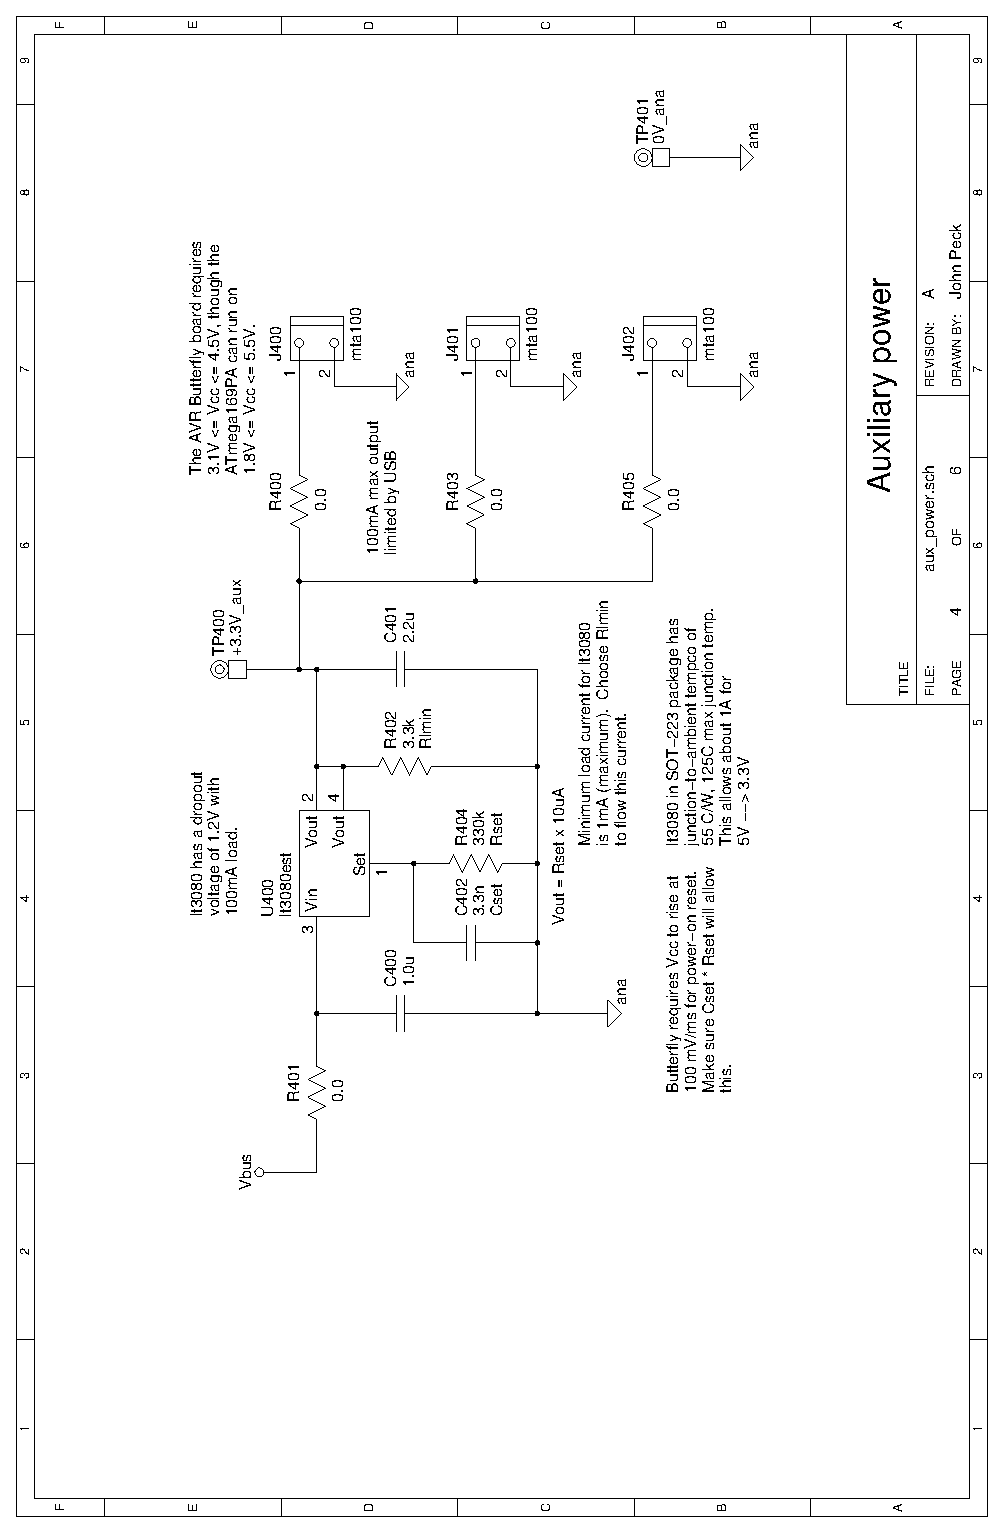
\includegraphics[clip,height=\textheight]
          {schematics/usb/aux_power}
          \label{sch:aux_power}
    \end{center} 
\end{figure}

\begin{figure}[ht]
    \begin{center}
          \vspace{0.4cm}
          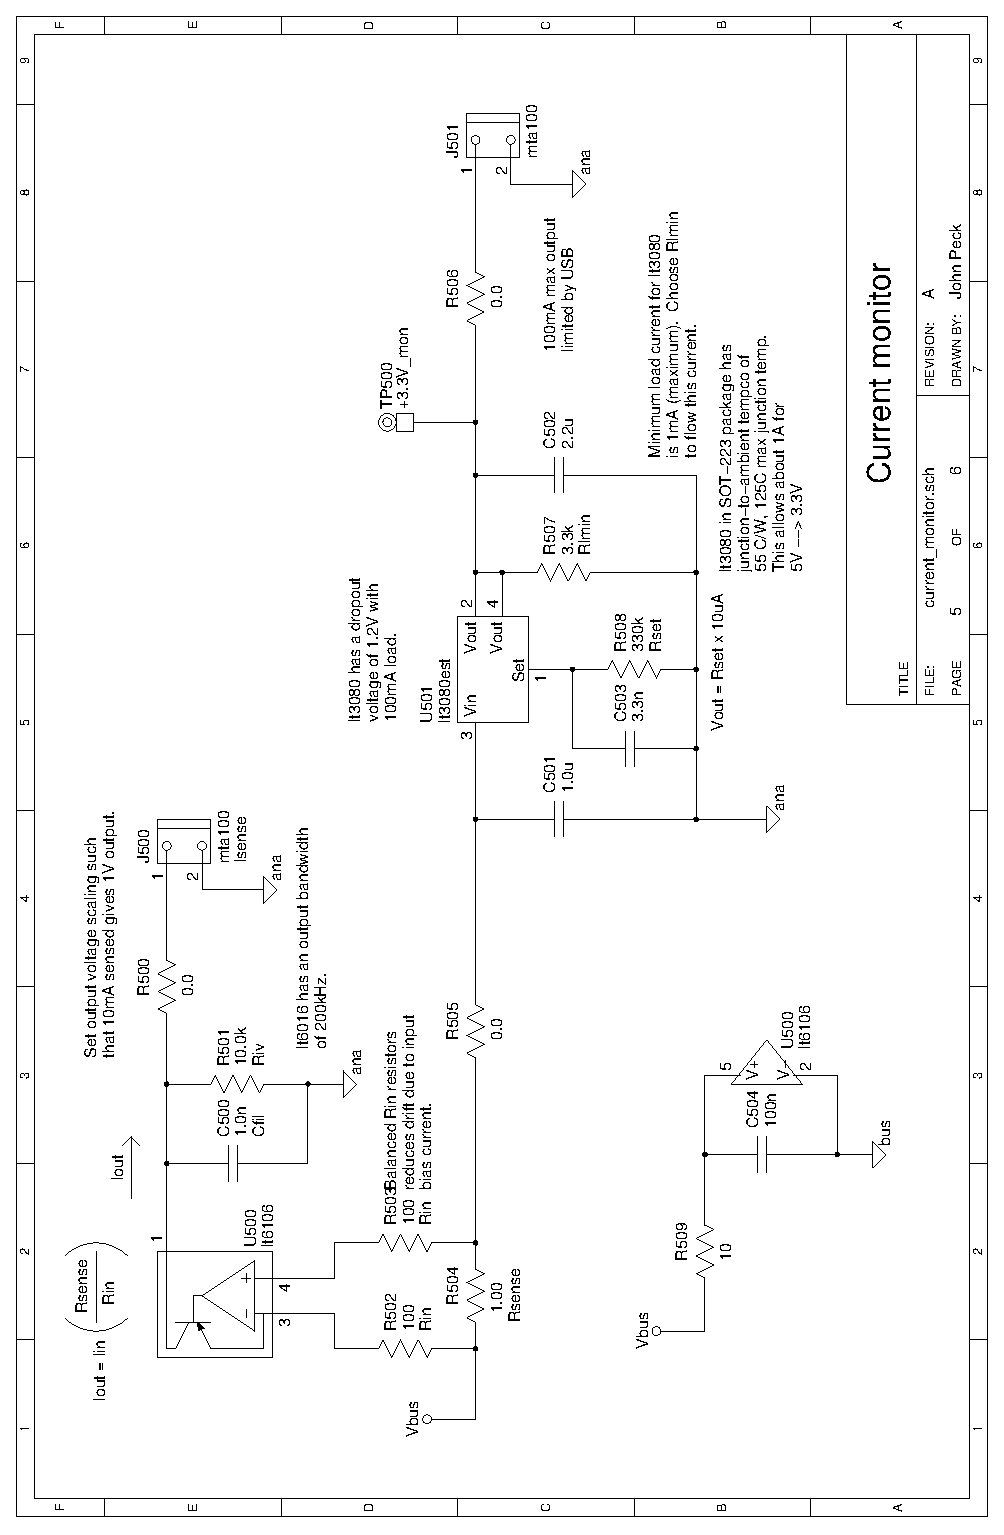
\includegraphics[clip,height=\textheight]
          {schematics/usb/current_monitor}
          \label{sch:current_monitor}
    \end{center} 
\end{figure}

\begin{figure}[ht]
    \begin{center}
          \vspace{0.4cm}
          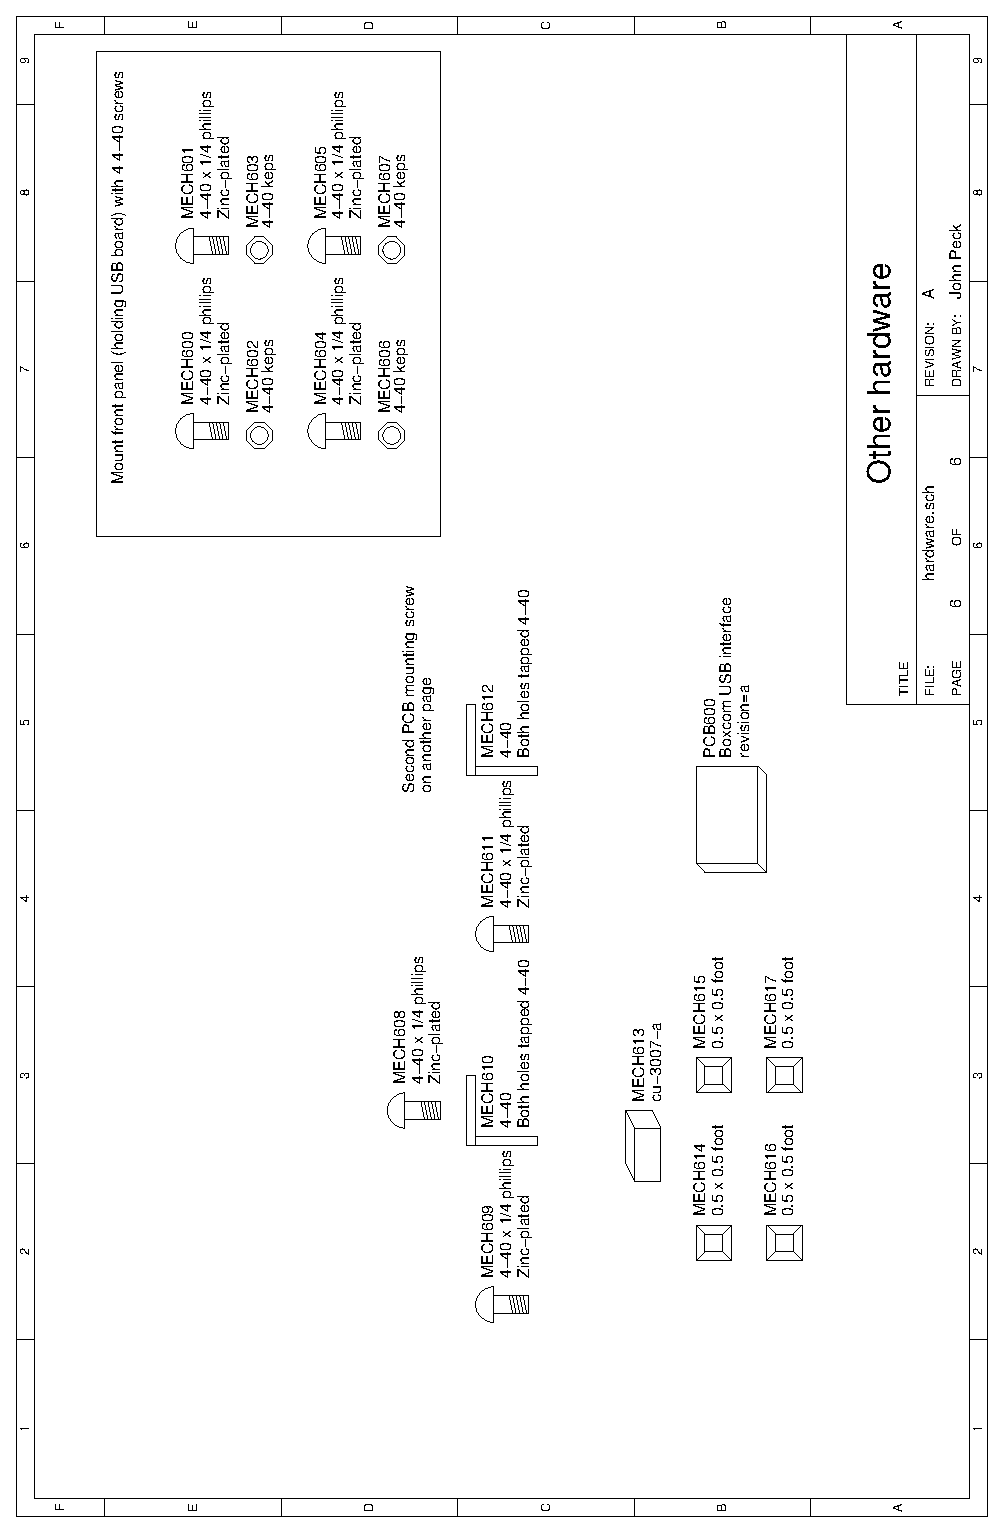
\includegraphics[clip,height=\textheight]
          {schematics/usb/hardware}
          \label{sch:hardware}
    \end{center} 
\end{figure}


%----------------------------------------------------------------------
% Bibliography
%
% 
%----------------------------------------------------------------------
\clearpage
% \addcontentsline{toc}{section}{Bibliography}
% \pagestyle{references} %set the references page style
% \bibliography{doctools/latex/ecrefs.bib}

















%%%%%%%%%%%%%%%%%%%%%%%%%%%%%%%%%%%%%%%%%%%%%%%%%%%%%%%%%%%%%%%%%%%%%%%%%%%
%Everything below here goes in the appendix
%%%%%%%%%%%%%%%%%%%%%%%%%%%%%%%%%%%%%%%%%%%%%%%%%%%%%%%%%%%%%%%%%%%%%%%%%%%
\appendix





%%%%%%%%%%%%%%%%%%%%%%%%%%%%%%%%%%%%%%%%%%%%%%%%%%%%%%%%%%%%%%%%%%%%%%%%%%%
% Indexes
%
%
%%%%%%%%%%%%%%%%%%%%%%%%%%%%%%%%%%%%%%%%%%%%%%%%%%%%%%%%%%%%%%%%%%%%%%%%%%%




% Redefine the printindex command to format the index in multiple columns.
% Uses the multicol package.  
% Don't try to use column separators (lines) -- there's still something
% strange going on with column widths.
%
% printindex still takes two arguments:
% 1. The ind file containing the index entries
% 2. The name for the index (will appear in the table of contents and at the
%    top of the index page.
\renewcommand{\printindex}[2]{
  % The \endtheindex command redefined by multind confounds the multicol
  % environment.  Redefine it to do nothing.  
  \renewcommand{\endtheindex}{}
  \addcontentsline{toc}{section}{#2}
  % Ideally, printindex would take an argument for the number of columns
  % instead of just hard coding it.
  \begin{multicols}{4}
    [\section*{#2}]
    \input{#1.ind}
  \end{multicols}
}% end printindex





% Alphabetical command index
\printindex{user_cmds_index}{Alphabetical command index}

%Internal SRS commands
\ifthenelse{\equal{\isforme}{1}}{
\clearpage{}
\printindex{internal_cmds_index}{Internal command index}
}{}



\end{document}
